\csname documentclass\endcsname[../main.tex]{subfiles}
\begin{document}
\chapter{Evaluation}

In this chapter, we evaluate the performance of our RLCEM. All experiments in this chapter
are conducted across multiple trials, where we report the mean
and standard deviation. This helps make our results statistically significant and reduces the errors
that arise from randomness, which is unavoidable in Machine
Learning experiments.
We compare our RLCEM which is a CEM augmented with an RL agent to learn 
a non-greedy intervention policy, to our baseline, which is IntCEM, and a number of other
heuristic-based intervention policies, 
including CooP that selects the 
concept which minimizes uncertainty, and Random that selects
random concepts to intervene on.

\section{Models and Datasets}\label{method:datasets}
% Brief description of each of these datasets and what they are each used for.
% Leave full description to be in appendix.
% Talk about concept groups
% Talk about subsampling
To evaluate the performance of our RLCEM model,
we follow Zarlenga et al.~\cite{intcem} and select the datasets MNIST-ADD and CUB for 
our experiments. Since these datasets have different input image sizes
and different number of possible classes,
the $\mathbf{x} \to \mathbf{c}$ and $\mathbf{c} \to \mathbf{y}$ models 
are slightly different, which we directly select the same 
models as Zarlenga et al.~\cite{intcem}
for a fair comparison. These CEM sub-models are kept the same
for RLCEM and the baseline IntCEM to ensure the results reflect a fair comparison 
of the learnt intervention policy.
Additionally for most of our ablation studies,
we conduct it on MNIST-ADD due to its straightforwardness.
For both datasets, 20\% of the training dataset is selected
as a validation dataset to monitor
the performance of the model during training. The validation dataset
is not used to update the model, but is rather used for 
hyperparameter selection and early stopping to prevent over-fitting.

\subsection{MNIST-ADD}
MNIST-ADD is a synthetic dataset created from 
the MNIST~\cite{mnist} dataset, a dataset of handwritten digits from 0 to 9.
The MNIST dataset contains black-and-white samples with an input size 
of $1 \times 28 \times 28$, and as shown in Table~\ref{table:datasets}, 
MNIST-ADD sample 
selects 12 images from the MNIST dataset as input $\mathbf{x}$,
with concepts corresponding to the values of each of the input images.
To model concept-incompleteness in real life datasetss,
which is when the 
concept annotations in the dataset may not contain all
possible concepts relevant, we select only the concepts corresponding to 8
of the input images, ensuring that the same conceps are selected across
all samples. This produces $54$ concepts which are then grouped into 8 
mutually-exclusive concept groups corresponding to images, 
and the label for each MNIST-ADD sample
is a binary label $\mathbf{y}$ corresponding to whether or not the sum of the input
12 images is greater than half of the possible maximum value.
 To generate the MNIST-ADD dataset,
we generate 10,000 training samples and 10,000 test samples by choosing
each of the 12 input images randomly from the MNIST training and testing
datasets respectively.

For this dataset, we use a ResNet-18~\cite{resnet} backbone for the $\mathbf{x} \to \mathbf{y}$
model with its output linear layer modified to 54 activations, corresponding
to the 54 concepts. The ResNet-18 backbone consists of 18 residual layers,
each containing two convolutional layers with batch normalization non-linear
activation functions, and is a popular backbone for image-related tasks.
The $\mathbf{c} \to \mathbf{y}$ model is an MLP with \{128, 128\} as the hidden
layers, and forwards the 54 predicted concepts to predict the binary label.

\subsection{CUB}

CUB~\cite{cub} is a real-life dataset that identifies bird attributes.
As shown in Table~\ref{table:datasets}, 
input $\mathbf{x}$ consist of $3 \times 299 \times 299$ images of 
 birds, and output $\mathbf{y}$ is a label representing the bird species.
We construct
112 annotation concepts 
using identifying features of birds such as their colour, shape, etc.,
then group it into 28 concept groups according
to Zarlenga et al~\cite{intcem}. We further group these
into 7 different concept groups for easy visualization and a better comparison
with MNIST-AFA. This also allows us to use the same RL models across datasets
as the size of the action space is simiar. There are 
5,994 training samples and 5,794 testing samples, which we fully
utilise during training and testing.

For this dataset, we use a ResNet-34~\cite{resnet} backbone for the 
$\mathbf{x} \to \mathbf{c}$
model with its output linear layer modified to 112 activations, corresponding
to the 112 concepts. The ResNet-34 uses the same layers as ResNet-18
with more layers deigned to process larger and more complicated images,
which we select due to the larger and more complex images in the CUB dataset.
The $\mathbf{c} \to \mathbf{y}$ model is an MLP with \{128, 128\} as the hidden
layers, and forwards the 112 predicted concepts to predict the label out of 200 classes.
% \subsection{CelebA}

% CelebA is another synthetic dataset constructed from 
% the popular CelebA dataset, a dataset that identifies celebrity face attributes.

\begin{table}
    \centering
    \renewcommand{\arraystretch}{1.5}
    \begin{tabular}{c|cc}
    % Dataset & Training Samples & Test Samples & Input Size & Concepts (k) & 
    % Concept Groups (n) & Output classes \\
    % \hline
    % MNIST-ADD & 10,000 & 10,000 & [12,28,28] & 54 & 8 & 2 \\
    % CUB & 5,994 & 5,794 & [3,299,299] & 112 & 28 & 200

    Dataset & MNIST-ADD & CUB \\
    \hline
    Training Samples & 10,000 & 5,994 \\
    Testing Samples & 10,000 & 5,794 \\
    Input Size & [12,28,28] & [3,299,299]\\
    Concepts (k) & 54 & 112 \\
    Concept Groups (n) & 8 & 7 \\
    Output classes & 2 & 100
    \end{tabular}
    \caption{The datasets and tasks used in this project.}
    \label{table:datasets}
\end{table}

More details on the datasets used can be found at Appendix~\ref{appendix:datasets}.

\subsection{Evaluating Performance}


\subsection{Reinforcement Learning Agent Model}
We adopt the same MLP for 
both the Actor and Critic model in the RL agent. 
We use the same number of layers as the intervention policy
 MLP used in IntCEM, but increase the number of neurons in the hidden layers
 to \{512, 512, 256, 256\} from \{128, 128, 64, 64\} as
 our problem is more complex, requiring 
 learning $O(n^2)$ tasks instead of $O(n)$ ($O(n)$ 
steps per budget for $O(n)$ different budgets).
 The same model is used
 for all datasets as the number of concept groups for intervention,
 which corresponds to the action space,
 is similar. We find that increasing the number of hidden layer neurons
 in the MLP used by 
 IntCEM to \{512, 512, 256, 256\} does not have any noticeable improvements
 to the intervention performance
 on a validation set.
    
\section{Non-greedy policies}

Before evaluating the performance of RLCEM, it is important to test whether or not 
non-greedy policies can outperform greedy policies. 
Therefore we conduct an
ablation study on the MNIST-ADD dataset, comparing two policies:
GreedyOptimal and TrueOptimal.
These are both the optimal policies,
i.e. the policies that select the concepts to intervene
on that lead to the highest accuracy. During 
testing, both of these policies have access to the true label $\mathbf{y}$, which 
allows them to find the concepts to intervene on 
such that the output
$\hat{\mathbf{y}} = \hat{g}(\hat{\mathbf{c}})$ 
has the highest accuracy.

While GreedyOptimal searches for the best concept group
out of all remaining un-intervened groups
to select at each step, TrueOptimal searches through
all possible combinations of concept groups to intervene at each budget, yielding
a time complexity of $O(n!)$ rather than
$O(n)$. This is also why while IntCEM can 
train a greedy intervention policy model directly
by training it to mimic the behaviour of a Greedy Optimal 
policy, it is infeasible to train a non-greedy intervention policy
model to mimic the behaviour of a True Optimal policy.

GreedyOptimal and TrueOptimal represent the theoretical
upper bound intervention performance
that greedy and non-greedy policies can achieve,
and we compare the two to see if the optimal 
non-greedy intervention policy can outperform the 
optimal greedy
intervention policy.

We train an IntCEM according to Zarlenga et al.~\cite{intcem}, 
and evaluate the intervention performance when using
GreedyOptimal and TrueOptimal. 

\begin{figure}[!h]
    \centering
    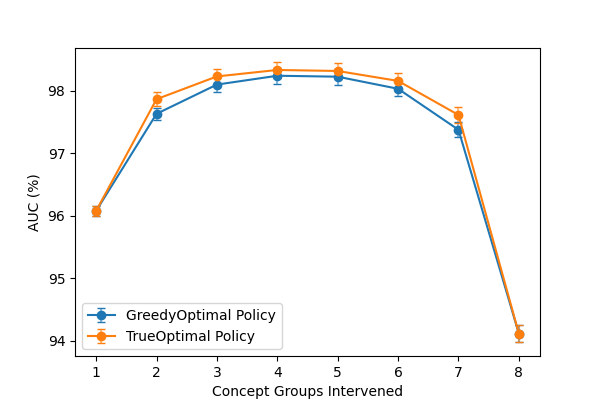
\includegraphics[width=0.9\textwidth]{figs/evaluation/greedy_vs_true_optimal.png}
    \caption{
        Intervention AUC on test set of using GreedyOptimal and TrueOptimal
        on an IntCEM trained on MNIST-ADD.
    }
    \label{fig:greedy-vs-optimal}
\end{figure}

Figure~\ref{fig:greedy-vs-optimal} shows the test performance of 
GreedyOptimal and TrueOptimal on an IntCEM
trained on MNIST-ADD. We see that TrueOptimal outperforms 
GreedyOptimal for all intervention groups, except
when only 1 group is intervened and when 8 groups are intervened
since the non-greedy and greedy optimal policies 
makes the same interventions for these two scenarios. 
The reason the performance when using
less interventions (eg. when 4 groups are intervened) is higher than
when more groups are intervened (eg. when all groups are intervened)
is because the intervention policies have access to the true 
label, and can cherry-pick interventions that result in 
the prediction to align more with the true label. This is
normal for a policy that has access to the 
true labels, and as we can see in 
Section~\ref{eval:rlcem-performance}, this behaviour is not observed 
in learnt policies such as IntCEM or RLCEM.


% \begin{table}
%     \centering
%     \begin{tabular*}{width}[pos]{cols}
        
%     \end{tabular*}
%     \caption{Performance of GreedyOptimal vs TrueOptimal }
% \end{table}

\section{Surrogate Models}\label{eval:surrogate}

We then look into the training of the 
surrogate models, which are used to model the conditional
likelihoods $p(\mathbf{c}_u \mid \mathbf{c}_o,y \mathbf{y})$ and used 
to provide intermediate rewards to the RL agent.
As mentioned in Section~\ref{method:surrogate}, 
we train the AC Flow model
using a negative log likelihood loss and a cross
entropy loss. The trained AC Flow model
will be frozen and used in the RLCEM model
to provide intermediate rewards to the RL agent.

To evaluate the performance of a trained 
AC Flow model, we look at 
its negative log likelihood and its accuracy on a validation set.
The accuracy is its accuracy in predicting 
the label $\hat{\mathbf{y}}$ which is given by 
\[\hat{\mathbf{y}} = \mathrm{\mathop{argmax}}_{\mathbf{y}} \;
p(\mathbf{c}_u \mid \mathbf{c}_o, \mathbf{y})\]
whereas the negative log likelihood (NLL) is the 
negative log likelihood of 
$p(\mathbf{c}_u \mid \mathbf{c}_o, \mathbf{y})$
for concepts $\mathbf{c}_u$ and $\mathbf{c}_o$ 
present in the validation dataset. We stop training if the validation loss
does not improve over several epochs, a common tactic used
to avoid over-fitting.

\begin{figure}[!h]
    \centering
    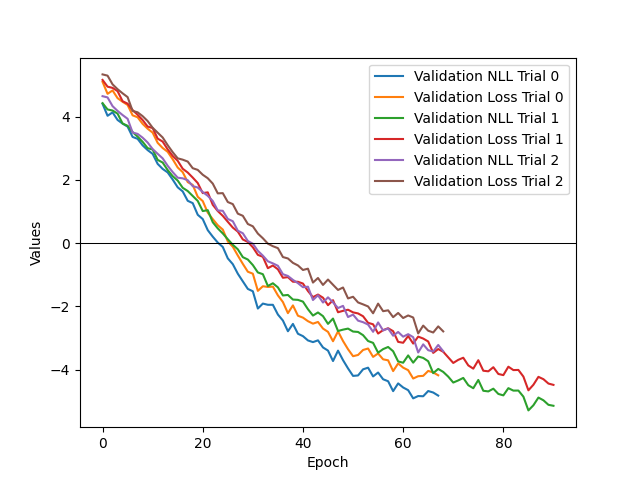
\includegraphics[width=0.7\textwidth]{figs/evaluation/mnist_acflow_no_val_accuracy_no_l2_loss_nll.png}
    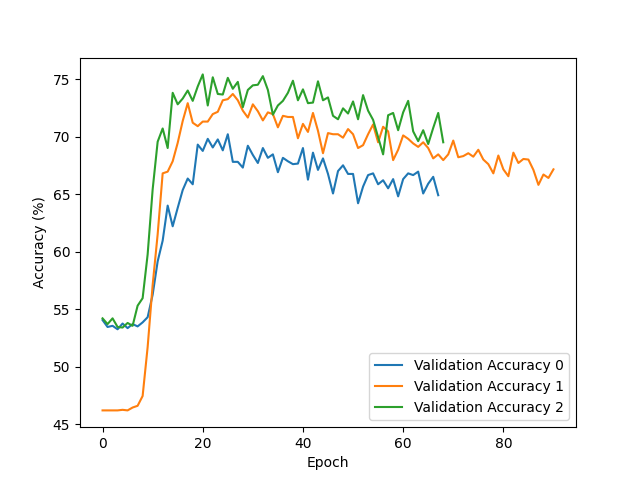
\includegraphics[width=0.7\textwidth]{figs/evaluation/mnist_acflow_no_val_accuracy_no_l2_accuracy.png}
    \caption{
        Performance on Validation Set when training an AC Flow model
        on the MNIST-ADD dataset across 3 trials.
        Top: Validation NLL and loss. Bottom: Validation Accuracy.
    }
    \label{fig:mnist-acflow-no-val-accuracy-no-l2-loss}
\end{figure}

Figure~\ref{fig:mnist-acflow-no-val-accuracy-no-l2-loss} shows the 
validation results when training an AC Flow model
on the MNIST-ADD dataset, using a learning-rate of 1e-6 and 
early stopping if validation loss does not improve over 5 epochs.
A large issue that we observe is that the validation loss
keeps decreasing and there seems to be no limit on when it stops.
This is because the model learns to output the log likelihoods 
of $p(\mathbf{c}_u \mid \mathbf{c}_o, \mathbf{y})$, and the underlying
model is a Gaussian Mixture Model which learns to output
a probability density at each value. While these probability densities,
at every point tells us the likelihood of that point,
it does not output an absolute probability with values in $[0,1]$. Therefore
the log likelihood can fall outside of $[-\infty, 0]$, and contain 
positive values, which is translated to a negative NLL and negative loss.
As the model keeps training, the model learns to output larger and larger
values for the more probable likelihoods, and the NLL keeps decreasing
to below 0, and the model does not appear to be able to stop as there is no
upper limit to the values it can output (and no lower limit to the NLL and hence
loss). At the same time we can see that the validation accuracy stops improving
after around 20 epochs and deteriorates, indicating that the model is over-fitting
long before validation loss starts to converge.
As a result, we use the validation accuracy as the early stopping
metric to prevent over-fitting. This helps ensure that 
the model learns about the underlying distribution and 
the log likelihood values accurately reflect the likelihood 
of concepts, which is 
shown from the validation accuracy, while preventing 
the output log likelihood values from growing endlessly, which
as we can see in Section~\ref{eval:rlcem-performance}, 
leads to other issues.

\section{RLCEM Performance}\label{eval:rlcem-performance}

\subsection{MNIST-ADD}

After training the AC Flow model on the MNIST-ADD dataset 
as illustrated in the previous section, we train RLCEM by 
using the
pretrained AC Flow model to provide intermediate rewards equal to 
the increase in information to the target as mentioned in 
Section~\ref{method:rlcem}.

\begin{figure}[!h]
    \centering
    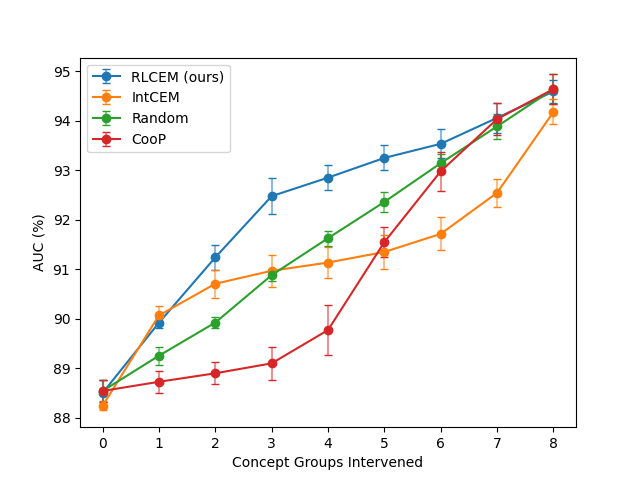
\includegraphics[width=0.9\textwidth]{figs/evaluation/mnist_rlcem_performance.png}
    \caption{
        Intervention AUC (\%) of RLCEM intervention
    policy compared to existing intervention policies.
    }
    \label{fig:mnist-performance-no-l2}
\end{figure}


\begin{table}
    \centering
    \renewcommand{\arraystretch}{1.5}
    \begin{tabular}{c|ccccc}
        \begin{tabular}{@{}c@{}}Concept Groups \\ Intervened\end{tabular} & RLCEM (Ours) & IntCEM & CooP & Random \\
    \hline
    $0\%$ & $\mathbf{88.2} \pm 0.3$ & $\mathbf{88.24} \pm 0.09$ & $\mathbf{88.24} \pm 0.09$ & $\mathbf{88.24} \pm 0.09$ \\
    $25\%$ & $\mathbf{91.1} \pm 0.4$ & $\mathbf{90.7} \pm 0.3$ & $88.7 \pm 0.2$ & $89.55 \pm 0.08$ \\
    $50\%$ & $\mathbf{93.2} \pm 0.2$ & $91.1 \pm 0.3$ & $91.1 \pm 0.2$ & $91.24 \pm 0.07$ \\
    $75\%$ & $\mathbf{94.0} \pm 0.2$ & $91.7 \pm 0.3$ & $93.4 \pm 0.2$ & $92.7 \pm 0.2$ \\
    $100\%$ & $\mathbf{94.5} \pm 0.4$ & $\mathbf{94.2} \pm 0.3$ & $\mathbf{94.2} \pm 0.3$ & $\mathbf{94.2} \pm 0.3$ \\
    \end{tabular}
    \caption{Intervention AUC (\%) of RLCEM intervention
    policy compared to existing intervention policies, higher is better. We highlight the 
    best performing policy in each row and values within 1 standard deviation.}
\end{table}

\subsection{CUB}

\section{Limitations}

\end{document}